\chapter{Southwestern Atlantic Cyclones Energetics} \label{ch:energetics}

The current chapter delves into the energetics of cyclones in the Southwestern Atlantic. The Lorenz Energy Cycle (LEC) was computed for all 7,531 systems with genesis in the ARG, LA-PLATA and SE-BR regions, as described in Chapter \ref{cyclone_life_cycle}. This is the first time such large dataset is generated and analysed for the South Atlantic region, providing a comprehensive view of the energetics of all systems with genesis near South America.

\textbf{CONTINUE}


1. \textbf{Descriptive Statistics}
    - Compute summary statistics (mean, median, standard deviation, skewness, and kurtosis) for each component of the Lorenz Energetics.
    - Create histograms and boxplots to visualize the distribution of these components.

2. \textbf{Comparative Analysis}
    - Seasonal Variations: Analyze how the Lorenz Energetics vary across different seasons. Use ANOVA or Kruskal-Wallis tests to determine if there are significant differences between seasons.
    - Geographical Differences: Assess the spatial variability of the energetics. You can use spatial clustering methods or geostatistical analysis to identify patterns.

3. \textbf{Trend Analysis}
    - Conduct time-series analysis to identify any long-term trends in the energetics components over the study period.
    - Use techniques like Mann-Kendall trend test or linear regression to assess the presence of trends.

4. \textbf{Correlation Analysis}
    - Examine the relationships between different components of the Lorenz Energetics (e.g., Ca x Ce, Residuals x Generation terms).
    - Use Pearson or Spearman correlation coefficients to quantify the strength and direction of these relationships.

5. \textbf{Principal Component Analysis (PCA)}
    - Perform PCA to reduce the dimensionality of the Lorenz Energetics data and identify the main modes of variability.
    - Interpret the principal components to understand the dominant patterns in the energetics data.

6. \textbf{Cluster Analysis}
    - Apply clustering techniques like K-means or hierarchical clustering to group cyclones based on their energetics profiles.
    - Analyze the characteristics of each cluster to identify distinct types of cyclones in terms of their energetics.

7. \textbf{Extreme Value Analysis}
    - Focus on the tails of the distribution to study extreme events.
    - Use generalized extreme value (GEV) distribution or peaks-over-threshold (POT) methods to model and analyze the extreme values of the energetics components.

8. \textbf{Hypothesis Testing}
    - Formulate and test hypotheses regarding the differences in Lorenz Energetics between different cyclone categories (e.g., intense vs. weak cyclones, coastal vs. open ocean cyclones).
    - Use t-tests, Mann-Whitney U tests, or chi-square tests depending on the data distribution and sample size.

9. \textbf{Multivariate Regression Analysis}
    - Build regression models to predict the Lorenz Energetics components based on various meteorological and oceanographic predictors.
    - Evaluate the model performance using metrics like R-squared, RMSE, and AIC.



\section{LEC Climatology}\label{sec:climatology}

\subsection{Descriptive Statistics: Complete Life Cycle} \label{sec:statistics_complete}

This section provides exploratory statistics for each term of the LEC, covering the systems' complete life cycle. The aim is to offer a comprehensive view of the systems' energetics while identifying the main differences among the terms. Table \ref{tab:lec_stats} contains exploratory statistical metrics for these terms. Figure \ref{fig:boxplot_energy_total} presents the boxplots for all LEC components, where each panel depicts a distinct group of terms: (A) energy, (B) conversion, (C) boundary, (D) generation/dissipation terms, and (E) budgets. Figures \ref{fig:ridge_plot_Energy_Terms_total}, \ref{fig:ridge_plot_Conversion_Terms_total}, \ref{fig:ridge_plot_Boundary_Terms_total}, \ref{fig:ridge_plot_Generation_Dissipation_Terms_total}, and \ref{fig:ridge_plot_Budgets_total} display these groups of terms' density distributions, respectively.

\begin{figure}[!htbp]
\centering
\includegraphics[width=32pc]{figs_5/box_plot_Total_all_groups.png}
\caption[Box plots - Complete Lifecycle]{Box plots of each group of energetic terms, for the systems complete lifecycle. Each subplot represents a different group of terms: (A) Energy Terms, (B) Conversion Terms, (C) Boundary Terms, (D) Generation/Dissipation Terms, (E) Budgets. The box plots display the distribution of values for each term within the specified group, with the horizontal line indicating the median, the box representing the interquartile range (IQR), and the whiskers extending to 1.5 times the IQR. Outliers are shown as individual points.}
\label{fig:boxplot_energy_total}
\end{figure}

For the energy terms, the values for $K_Z$ are an order of magnitude higher than the others for all metrics analyzed (Table \ref{tab:lec_stats}). Despite the high standard deviation (std) and quantile (Q) values indicating substantial variability, this can be attributed to the presence of numerous outliers (Figure \ref{fig:boxplot_energy_total}a). Most values for $K_Z$ peak between 15 and 17 $\times 10^5 \, J \, m^{-2}$ (Figure \ref{fig:ridge_plot_Energy_Terms_total}c). In contrast, $A_Z$ presents relatively moderate mean and median values, with a right-skewed distribution and significant spread (Figure \ref{fig:ridge_plot_Energy_Terms_total}a). The notable outliers (Figure \ref{fig:boxplot_energy_total}a) suggest periods of unusually high energy values.

Overall, the eddy energy terms ($A_E$ and $K_E$) exhibit less variability and fewer outliers compared to the zonal energy terms ($A_Z$ and $K_Z$) (Figure \ref{fig:boxplot_energy_total}a). They also have smaller mean and median values (Table \ref{tab:lec_stats}). Although both eddy energy terms peak close to each other, the distribution of $A_E$ is more concentrated around the median (Figure \ref{fig:ridge_plot_Energy_Terms_total}b), with a narrower interquartile range (IQR) and lower standard deviation, suggesting it is more stable and consistent over time. In contrast, $K_E$ presents a more right-skewed distribution than $A_E$ (Figure \ref{fig:ridge_plot_Energy_Terms_total}d).


\begin{figure}[!htbp]
\centering
\includegraphics[width=32pc]{figs_5/ridge_plot_Energy_Terms_total.png}
\caption[Density Plots - Energy Terms]{Density plots for energy terms $A_Z$ (A), $A_E$ (B), $K_Z$ (C), and $K_E$ (D). Each subplot represents the distribution of values for the specified energy term, showing the density across different value ranges.}
\label{fig:ridge_plot_Energy_Terms_total}
\end{figure}

While the mean values of $A_E$ and $K_E$ are generally in agreement with previous studies, the values of $K_Z$ and $A_Z$ differ significantly \citep[e.g.,]{michaelides1999quasi,veiga2008analysis,dias2011energy,pezza2014large}. \citet{li2007lorenz} and \citet{veiga2013global}, analyzing global LEC values, found mean $K_Z$ values for the Southern Hemisphere of approximately $10$ and $15.8 \times 10^5 \, J \, m^{-2}$ and mean $A_Z$ values of approximately $40$ and $16 \times 10^5 \, J \, m^{-2}$, respectively. Analyzing the LEC of extratropical cyclones primarily in the Northern Hemisphere, \citet{smith1980energetics} found mean $K_Z$ and $A_Z$ values of $15$ and $25 \times 10^5 \, J \, m^{-2}$, respectively. Meanwhile, \citet{black2013universal}, for explosive cyclogenesis in the Northwest Pacific region, found mean $A_Z$ and $K_Z$ values of approximately $30$ and $48 \times 10^5 \, J \, m^{-2}$, respectively. Here, $K_Z$ and $A_Z$ presented mean values of $28.55$ and $5.55 \times 10^5 \, J \, m^{-2}$, respectively.


\begin{table}[!htbp]
\centering
\caption[Summary Statistics of Lorenz Energetics Components]{Summary Statistics of Lorenz Energetics Components: mean, median, standard deviation (std), 20th percentile (Q20), 80th percentile (Q80), interquantile range (IQR), and range. The IQR measures the range within which the central 50\% of the values fall, while the range is computed as the difference between the maximum and minimum values. The units for the energy terms ($A_Z$, $A_E$, $K_Z$, and $K_E$) are $10^5 \, J \, m^{-2}$ and $W \, m^{-2}$ for the remaining terms.}
\label{tab:lec_stats}
\begin{tabular}{lrrrrrrr}
\toprule
Term & Mean & Median & Std & Q20 & Q80 & IQR & Range \\
\midrule
Az & 5.55 & 4.68 & 3.71 & 2.41 & 8.30 & 5.89 & 36.46 \\
Ae & 1.62 & 1.24 & 1.20 & 0.69 & 2.37 & 1.68 & 11.07 \\
Kz & 28.55 & 26.19 & 15.10 & 15.52 & 40.16 & 24.64 & 114.55 \\
Ke & 3.70 & 2.95 & 2.62 & 1.73 & 5.22 & 3.49 & 24.81 \\
Cz & 0.52 & 0.38 & 4.85 & -2.69 & 3.72 & 6.41 & 86.70 \\
Ca & 0.93 & 0.46 & 1.57 & -0.06 & 1.79 & 1.84 & 19.78 \\
Ck & -3.56 & -1.63 & 9.51 & -7.41 & 1.11 & 8.52 & 206.43 \\
Ce & 3.84 & 2.47 & 4.92 & 0.33 & 6.97 & 6.64 & 54.74 \\
BAz & 3.54 & 2.03 & 7.67 & -1.35 & 8.23 & 9.57 & 175.05 \\
BAe & 0.58 & 0.16 & 4.40 & -1.62 & 2.75 & 4.37 & 75.72 \\
BKz & -7.93 & -5.53 & 31.75 & -29.51 & 12.06 & 41.57 & 445.63 \\
BKe & 0.47 & 0.08 & 8.59 & -3.67 & 4.40 & 8.07 & 146.87 \\
$B\Phi Z$ & 63.87 & 49.25 & 128.05 & -24.60 & 156.65 & 181.25 & 1419.08 \\
$B\Phi E$ & 39.66 & 31.19 & 126.50 & -46.44 & 132.10 & 178.54 & 1353.99 \\
Gz & -0.31 & -0.17 & 2.66 & -1.82 & 1.14 & 2.96 & 68.74 \\
Ge & 1.17 & 0.56 & 3.14 & -0.47 & 2.79 & 3.26 & 58.39 \\
$\frac{\partial A_Z}{\partial t}$ & -0.07 & -0.14 & 4.46 & -2.66 & 2.31 & 4.97 & 106.39 \\
$\frac{\partial A_E}{\partial t}$ & -0.23 & -0.10 & 1.92 & -1.14 & 0.74 & 1.88 & 48.19 \\
$\frac{\partial K_Z}{\partial t}$ & 1.59 & 0.75 & 13.38 & -7.13 & 10.40 & 17.53 & 251.24 \\
$\frac{\partial K_E}{\partial t}$ & 0.28 & 0.12 & 3.18 & -1.53 & 2.09 & 3.62 & 61.50 \\
RGz & -2.17 & -1.00 & 7.60 & -6.69 & 2.31 & 9.01 & 220.06 \\
RKz & 12.56 & 8.69 & 40.49 & -13.89 & 40.08 & 53.96 & 561.24 \\
RGe & 2.10 & 1.20 & 5.15 & -0.84 & 5.28 & 6.12 & 97.25 \\
RKe & -7.59 & -4.63 & 10.62 & -13.68 & -0.45 & 13.23 & 138.42 \\
\bottomrule
\bottomrule
\end{tabular}
\end{table}

The scarcity of results for a comprehensive set of systems hinders drawing decisive conclusions about the behavior of the $A_Z$ and $A_E$ terms in cyclonic occurrences, while individual cases offer high variability, as indicated by case studies \citep[e.g.,]{brennan1980zonal,dias2011energy,pezza2014large} and the higher variability in the data (Table \ref{tab:lec_stats}). However, several observations can be made:  1) When compared to global energetics, cyclonic systems present higher $K_Z$ values. This is expected because $K_Z$ involves a zonal average of the wind components (Equation \ref{eq:KZ}), and global averages would yield smaller values than those for limited areas closer to the cyclonic center, often associated with high-level jets; 2) Limited areas provide smaller $A_Z$ values than hemispheric averages, due to the reduced meridional temperature and static stability gradients (Equation \ref{eq:AZ}). These effects are even more evident in the current study, as the computational domain following the system focuses on the environmental dynamics surrounding it, thus capturing overall higher wind speeds through the atmosphere and smaller meridional temperature gradients. A similar effect is noted in \citet{michaelides1999quasi}; 3) Furthermore, the literature shows that the magnitude and sign of the conversion, boundary, generation, and dissipation terms exhibit high variability across different systems and development phases \citep[e.g.,]{brennan1980zonal,smith1980energetics,michaelides1987limited,bulic2006limited,dias2011energy,black2013universal}, complicating comparisons of the overall values presented here with individual cases.

For the conversion terms, while $C_Z$, $C_A$, and $C_E$ are positive on average and in median values, $C_K$ is negative (Table \ref{tab:lec_stats}). For $C_A$ and $C_E$, there is a relatively narrow spread around the median, with some significant outliers (Figure \ref{fig:boxplot_energy_total}b). $C_A$, showing a distribution centered around zero with both negative and positive values (Figure \ref{fig:ridge_plot_Conversion_Terms_total}b), indicates alternating periods of energy transfer in both directions, predominantly from $A_Z$ to $A_E$. Meanwhile, $C_E$ has a left-skewed distribution (Figure \ref{fig:ridge_plot_Conversion_Terms_total}d) and higher Q20 and IQR values, suggesting a more consistent positive net conversion. 

The $C_K$ term exhibits a wide distribution peaking at negative values (Figure \ref{fig:ridge_plot_Conversion_Terms_total}c), with a significant negative mean and median, indicating a dominant net conversion from $K_Z$ to $K_E$. The large range and standard deviation, along with the presence of significant outliers, suggest substantial variability in this conversion process. Lastly, $C_Z$ presents the most distinctive behavior, with values centered around zero but peaking at both positive and negative values (Figure \ref{fig:ridge_plot_Conversion_Terms_total}a). However, the higher peak at positive values along with the positive mean and median values indicate a preference for conversion from $A_Z$ to $K_Z$. 

The overall values presented here indicate that, throughout the systems' complete lifecycle, $K_E$ tends to receive energy from $A_E$ and, in most cases, from $K_Z$ as well, although there are instances where $C_K$ tends to be positive. There is also a general tendency for $A_Z$ to be converted to $A_E$, albeit with a lower magnitude. Meanwhile, although $C_Z$ can be positive, negative, or neutral, the predominant tendency is for conversion from $A_Z$ to $K_Z$.

\begin{figure}[!htbp]
\centering
\includegraphics[width=32pc]{figs_5/ridge_plot_Conversion_Terms_total.png}
\caption[Density Plots - Conversion Terms]{Density plots for conversion terms $C_Z$ (A), $C_A$ (B), $C_K$ (C), and $C_E$ (D). Each subplot represents the distribution of values for the specified energy term, showing the density across different value ranges.}
\label{fig:ridge_plot_Conversion_Terms_total}
\end{figure}

There is a notable difference between the boundary flux terms ($BA_Z$, $BA_E$, $BK_Z$, $BK_E$) and the boundary pressure work terms ($B\Phi Z$ and $B\Phi E$) (Table \ref{tab:lec_stats}). For the boundary flux terms, $BA_Z$ presents the highest mean and median values, while $BK_Z$ has the lowest. $BA_E$ and $BK_E$ have mean and median values closer to zero. The $BA_Z$ term exhibits moderate variability, with a wide distribution around the median (Figure \ref{fig:ridge_plot_Boundary_Terms_total}a) and few outliers (Figure \ref{fig:boxplot_energy_total}c), a similar pattern to $BK_E$ (Figure \ref{fig:ridge_plot_Boundary_Terms_total}d). $BA_E$, in turn, displays the lowest variability among the boundary terms, with most values peaking near zero (Figure \ref{fig:ridge_plot_Boundary_Terms_total}b). Meanwhile, $BK_Z$ presents the most distinctive behavior, exhibiting high variability, with a wide distribution (Figure \ref{fig:ridge_plot_Boundary_Terms_total}c) and numerous outliers. Its values range from the most negative to the most positive among the boundary terms, indicating an overall tendency for the exportation of zonal kinetic energy, supported by its negative mean and median values.

On the other hand, the boundary pressure work terms present similar behavior, with very high mean and median values, especially $B\Phi Z$, and displaying two peaks: one on negative values (with a higher peak for the $B\Phi E$ term) and another, which displays higher densities, on positive values (Figure \ref{fig:ridge_plot_Boundary_Terms_total}e and \ref{fig:ridge_plot_Boundary_Terms_total}f). Both terms present low Q20 and high Q80 values, indicating that although they generally contribute to the appearance of energy in the $K_Z$ and $K_E$ terms, there are instances where they contribute negatively. For all metrics presented, they exhibit the highest values in magnitude across all terms. As \citet{brennan1980zonal} argued, these high values are associated with minor errors in the geopotential height field that can escalate. Although ERA5 presents the most modern reanalysis product offering homogeneous high-resolution data, systematic errors might be present, especially in regions with low data coverage, such as over the oceans and high altitudes \citep{hersbach2020era5}. As most studies do not compute these terms as residuals and thus do not present the values (for instance, none of the studies presented in Section \ref{sec:lec_cyclones} do so), direct comparison of the values obtained here with the literature is hindered.

\begin{figure}[!htbp]
\centering
\includegraphics[width=32pc]{figs_5/ridge_plot_Boundary_Terms_total.png}
\caption[Density Plots - Boundary Terms]{Density plots for boundary terms $BA_Z$ (A), $BA_E$ (B), $BK_Z$ (C), $BK_E$ (D), $B\Phi Z$ (E), and  $B\Phi E$ (F). Each subplot represents the distribution of values for the specified energy term, showing the density across different value ranges.}
\label{fig:ridge_plot_Boundary_Terms_total}
\end{figure}

%% !
Although the energy budgets are computed using residuals (which include the boundary pressure work terms), the generation terms are also analyzed as they serve both as an overall evaluation of the generation residual terms and because, in future sections, they will be used for understanding the systems' dynamics. Both $G_Z$ and $G_E$ present a similar distribution, displaying low variability (Figure \ref{fig:ridge_plot_Boundary_Terms_total}), with most values peaking near zero and with minor peaks on both positive and negative values (Figures \ref{fig:ridge_plot_Generation_Dissipation_Terms_total}a and \ref{fig:ridge_plot_Generation_Dissipation_Terms_total}b). However, $G_E$ presents a higher density of positive values, which is reflected in its higher mean and median values than $G_Z$ and higher Q80 values (Table \ref{tab:lec_stats}). 

For the generation residual terms, both present three peaks - at positive, neutral, and negative values - but while $RG_Z$ has the highest density around negative values, $RG_E$ peaks at positive values (Figures \ref{fig:ridge_plot_Generation_Dissipation_Terms_total}c and \ref{fig:ridge_plot_Generation_Dissipation_Terms_total}e). This results in $RG_E$ presenting positive mean and median values, despite a minor peak at negative values - which reflects in a negative Q20 value - indicating that its contribution to $\frac{\partial A_E}{\partial t}$ is mainly positive, with situations where this term contributes negatively. For $RG_Z$, the opposite is noted, with negative mean and median values, but a minor peak at positive values - reflected in a positive Q80 - indicating it mainly contributes negatively to $\frac{\partial A_Z}{\partial t}$, with situations where this term contributes positively.

Furthermore, while $RK_Z$ presents higher positive mean and median values, it also shows high variability and numerous outliers (Figure \ref{fig:boxplot_energy_total}d). It presents a distinctive density distribution, with two marked peaks, one for positive and the other for negative values (Figure \ref{fig:ridge_plot_Generation_Dissipation_Terms_total}d). This is reflected in its negative Q20 and positive Q80 values, with a high IQR. Therefore, although it mostly contributes positively to $\frac{\partial K_Z}{\partial t}$, there are also significant instances where it contributes negatively. $RK_E$, on the other hand, presents mean and median values peaking at negative values (Figure \ref{fig:ridge_plot_Generation_Dissipation_Terms_total}f). Therefore, it mostly contributes negatively to $\frac{\partial K_E}{\partial t}$, acting as a sink for $K_E$.

\begin{figure}[!htbp]
\centering
\includegraphics[width=32pc]{figs_5/ridge_plot_Generation_Dissipation_Terms_total.png}
\caption[Density Plots - Generation Terms]{Density plots for generation terms $G_Z$ (A) and $G_E$ (B); and residual terms $RG_Z$ (C), $RK_Z$ (D), $RG_E$ (E), and $RK_E$ (F). Each subplot represents the distribution of values for the specified energy term, showing the density across different value ranges.}
\label{fig:ridge_plot_Generation_Dissipation_Terms_total}
\end{figure}

Among the budget terms, APE terms ($\frac{\partial A_Z}{\partial t}$ and $\frac{\partial A_E}{\partial t}$) present negative mean and median values, while the kinetic energy terms ($\frac{\partial K_Z}{\partial t}$ and $\frac{\partial K_E}{\partial t}$) are positive, although all of them exhibit negative Q20 values and positive Q80 values, indicating variability among the analyzed systems (Table \ref{tab:lec_stats}).  $\frac{\partial A_E}{\partial t}$ has the lowest variability, with the smallest IQR and range values, fewest outliers (Figure \ref{fig:boxplot_energy_total}), and the highest peak density centered around zero (Figure \ref{fig:ridge_plot_Budgets_total}b). This indicates that while in most cases there is an overall tendency for $A_E$ to be neutral, there are also occurrences of positive and negative increments.

In contrast, $\frac{\partial A_Z}{\partial t}$ and $\frac{\partial K_E}{\partial t}$ display similar density distributions (Figure \ref{fig:ridge_plot_Budgets_total}a and \ref{fig:ridge_plot_Budgets_total}d), with peaks at negative, neutral, and positive values. $\frac{\partial A_Z}{\partial t}$ has a higher peak at negative values, indicating a tendency for $A_Z$ to decrease, while $\frac{\partial K_E}{\partial t}$ peaks at positive values, reflecting a tendency for $K_E$ to increase. However, both terms also show instances of neutrality and opposite trends.

Lastly, $\frac{\partial K_Z}{\partial t}$ exhibits a unique behavior with two prominent peaks at opposite extremes (Figure \ref{fig:ridge_plot_Budgets_total}c). This term has the lowest Q20 and the highest Q80, IQR, and range values, indicating that $K_Z$ tends to exhibit extreme changes — either significant increases or decreases — with a smaller tendency to remain neutral.


\begin{figure}[!htbp]
\centering
\includegraphics[width=32pc]{figs_5/ridge_plot_Budgets_total.png}
\caption[Density Plots - Budget Terms]{Density plots for budget terms $\frac{\partial A_Z}{\partial t}$ (A) and $\frac{\partial A_E}{\partial t}$ (B); $\frac{\partial K_Z}{\partial t}$ (C), and $\frac{\partial K_E}{\partial t}$ (D). Each subplot represents the distribution of values for the specified energy term, showing the density across different value ranges.}
\label{fig:ridge_plot_Budgets_total}
\end{figure}

\subsection{EOFs}

The results presented in Section \ref{sec:statistics_complete} demonstrate that the LEC terms exhibit high variability: each term spans a wide range of possible values, often with varying signs. Therefore, delineating an overall picture of the LEC for the analyzed systems is not a trivial task. To address this issue, an EOF analysis is used (Figure \ref{fig:eofs_total}). It is important to note that the values represent anomalies rather than actual magnitudes of the energy cycle components. Additionally, $G_Z$ and $G_E$ terms are used for a more physically based interpretation, although the budgets were computed using their respective residuals. Since the residual terms integrated these components, the presented budgets may not perfectly balance positive and negative energy fluxes due to the finite differences method used, which also incorporates numerical errors.

The first EOF (EOF1, Figure \ref{fig:eofs_total}b) indicates an overall tendency for $A_Z$ to decrease over time, primarily due to conversions to $A_E$ ($C_A > 0$, Figure \ref{fig:Ca}), which is an expected result. As discussed in Section \ref{track_method}, most cyclones in the dataset are extratropical, which have the final cause of diminishing Equator-Pole temperature gradients (Section \ref{final_causes}), i.e., reducing $A_Z$. Additionally, there are losses of $A_Z$ due to the $G_Z$ term, indicating either anomalous heating in cool regions or anomalous cooling in warm regions caused by the eddy's meridional heat transport. Significant imports of $A_Z$ are also observed through the $BA_Z$ term. For the $A_E$ term, there are only negligible increases over time. Despite influxes from $C_A$ and diabatic processes ($G_E > 0$), most of its energy is converted to $K_E$ ($C_E > 0$) due to enhanced zonal temperature gradients, while some of it is exported from the domain ($BA_E < 0$).

EOF1 indicates $K_E$ increasing over time. This increase primarily stems from influxes from the residual term ($RK_E > 0$). Although the inclusion of numerical errors hinders the interpretation of the residual term, Section \ref{sec:climatology} indicates that $B\Phi_Z$ often presents large values, suggesting that this energy influx might be related to the generation of kinetic energy towards the cyclone's central low pressure. Meanwhile, part of $K_Z$ energy is exported outside the domain ($BK_Z < 0$) or converted to $K_E$ through the barotropic conversion term ($C_K < 0$). Only negligible amounts are converted into $A_Z$. Finally, $K_E$ displays increases over time, driven mostly by conversion from $A_E$, but also with significant contributions from $K_E$. Notably, $RK_E$ presents a similar magnitude to $C_E$, possibly indicating the dissipation of this energy. The importation of $K_E$ is almost negligible.

Overall, in terms of the mechanisms related to the eddy growth, it can be seen that for EOF1 both the baroclinic and barotropic chains were active. This indicates that the eddy was gaining energy from both meridional temperature gradients as well as from horizontal wind shear. Moreover, diabatic processes were contributing to increasing the eddy APE, thus contributing to the moist baroclinic chain. Finally, the main sink for eddy energy was the residual term, possibly associated with dissipation by frictional forces.

\begin{figure}[!htbp]
\centering
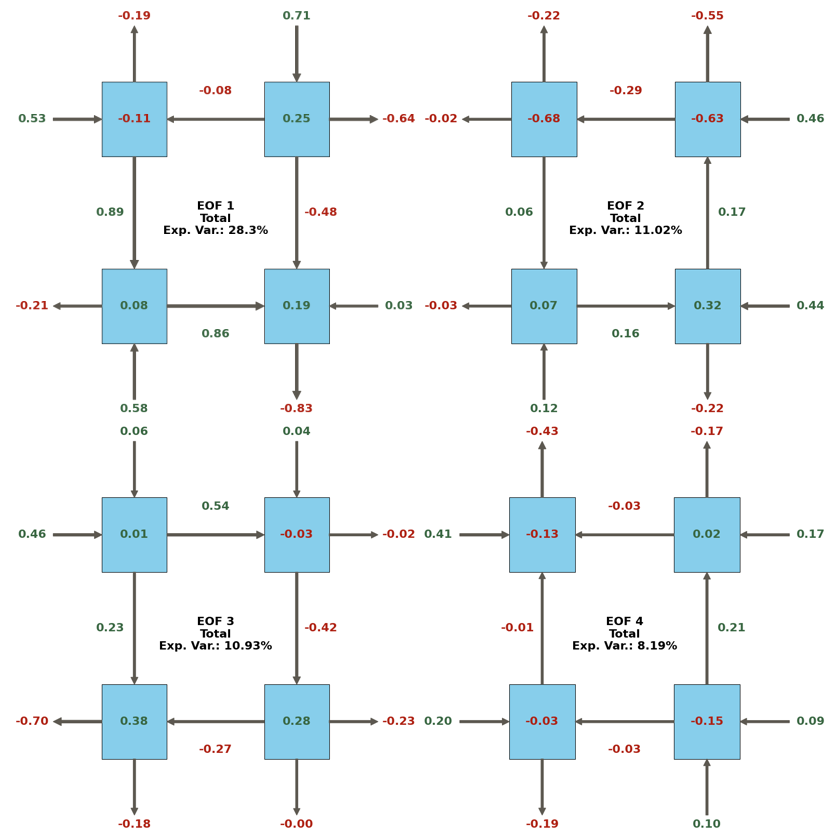
\includegraphics[width=32pc]{figs_5/eofs_total.pdf}
\caption[EOF Analysis - Total Lifecycle]{EOF Analysis of Lorenz Energy Cycle (LEC) Terms. The first diagram represents the LEC components, with each blue box indicating a specific energy component, with arrows showing the direction of energy flow. Meanwhile, the other diagrams represent the first three Empirical Orthogonal Functions (EOFs) of the energy cycle components, illustrating the anomalies in energy fluxes. 
The numbers adjacent to the arrows denote the magnitude and direction of the anomaly, with green indicating positive values and red indicating negative values.}
\label{fig:eofs_total}
\end{figure}



% \section{Limitações, aplicações e passos futuros}
% \begin{itemize}
%     \item Limitações: metodologia semi-lagrangiana deve ser interpretada como snapshots (relacionando com \citet{muench1965dynamics})
%     \item  A formulação adotada apenas permite a seguinte interpreteção: contribuição para energética global e não a energética individual de cada sistema
%     \item Contextualizar a energética como ferramenta para determinação objetiva das causas eficientes e finais dos ciclones (diagramas do Hart estão relacionados com causas formais e materiais - os trabalhos complementam-se)
%     \item Estudos de caso? (e.g. ciclones extratropicais clássicos formados no sul da ARG, ciclones bomba formados em LA-PLATA, ciclones subtropicais formados em SE-BR e, ciclones tropicais Anita, Iba, 01Q.
% \end{itemize}